\chapter{Training for Regression Using Energy Summed in z}\label{app:z_sum_regression}

For regression, we tried using only the energy summed in layers in the $z$ direction, instead of the full array of cell energies, as the mean $z$ coordinate was seen to be the most important additional feature in the XGBoost baseline.  The performance is better than the XGBoost baseline at high energies but worse than using the full cell-level information, as shown in Figure~\ref{fig:reg_dnn_inputs}.

\begin{figure}[htbp]
\centering
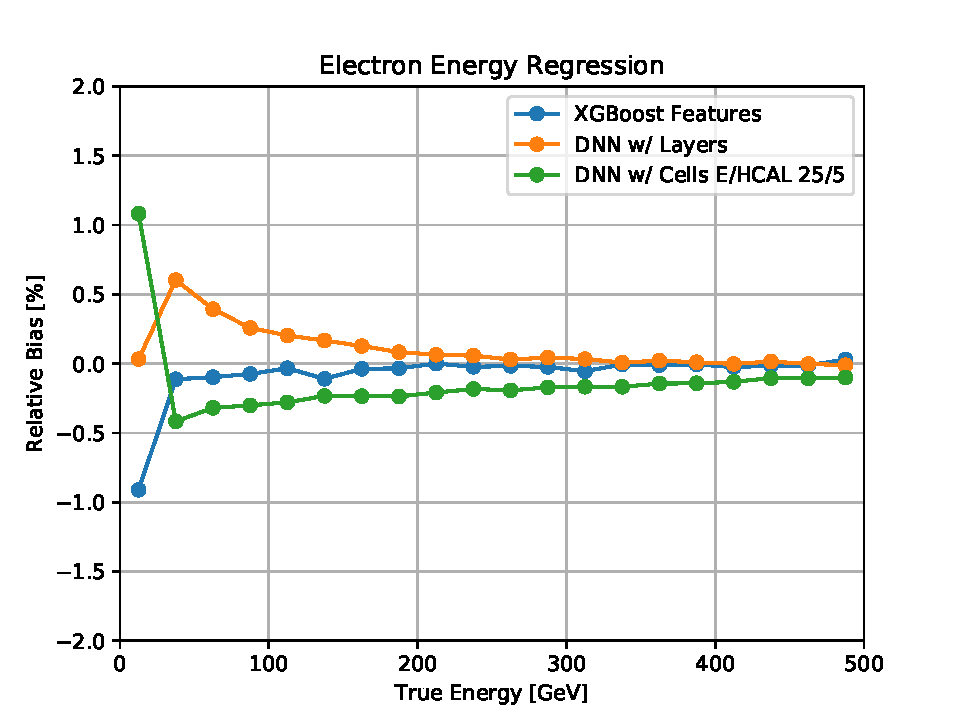
\includegraphics[width=0.38\textwidth]{Images/Calo/bias_vs_E_EleFixed_nn_inputs_zoom.pdf}
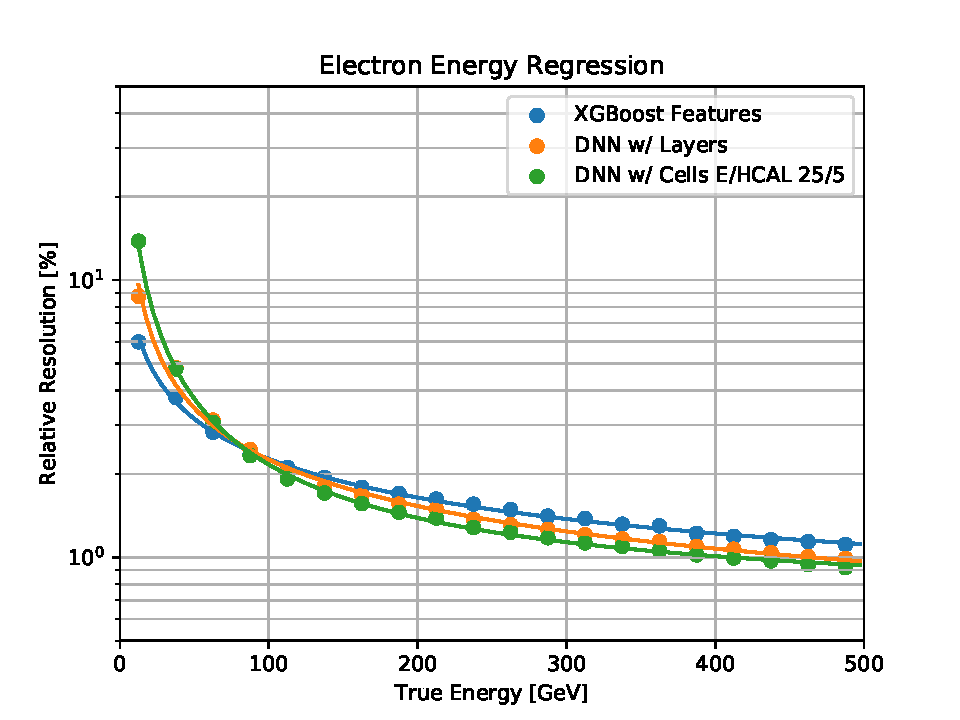
\includegraphics[width=0.38\textwidth]{Images/Calo/res_vs_E_EleFixed_nn_inputs_fits.pdf}
\caption{Bias (top) and resolution (bottom) as a function of true energy for DNN energy predictions for electrons, using as input either the energy summed in layers of $z$, or the full cell information.\label{fig:reg_dnn_inputs}}
\end{figure}